\subsection{Ordenamiento de Arreglos}

La \Cref{tab:sorting_summary} resume los tiempos promedio observados para los tamaños extremos ($N=10^5$ y $N=10^7$) en arreglos aleatorios, mientras que la \Cref{fig:sorting_plots} ilustra las curvas de rendimiento en escala logarítmica.

\begin{table}[H]
\centering
\caption{Tiempo de ejecución promedio (ms) para arreglos aleatorios ($N=10^5$ y $N=10^7$).}
\label{tab:sorting_summary}
\small
\begin{tabular}{lrrrr}
\hline
\textbf{Algoritmo} & \textbf{$N=10^5$ ($D_1$)} & \textbf{$N=10^5$ ($D_7$)} & \textbf{$N=10^7$ ($D_1$)} & \textbf{$N=10^7$ ($D_7$)} \\ \hline
\texttt{std::sort}    & 2.11 ms  & 5.19 ms  & 173.85 ms & 581.70 ms \\
MergeSort             & 3.58 ms  & 6.80 ms  & 382.94 ms & 837.80 ms \\
QuickSort             & 2.57 ms  & 6.54 ms  & 212.49 ms & 701.24 ms \\
PatienceSort          & 2.82 ms  & 7.42 ms  & 224.80 ms & 962.82 ms \\ \hline
\end{tabular}
\end{table}

\begin{figure}[H]
    \centering
    \subfloat[Aleatorio - Dominio $D_1$]{%
        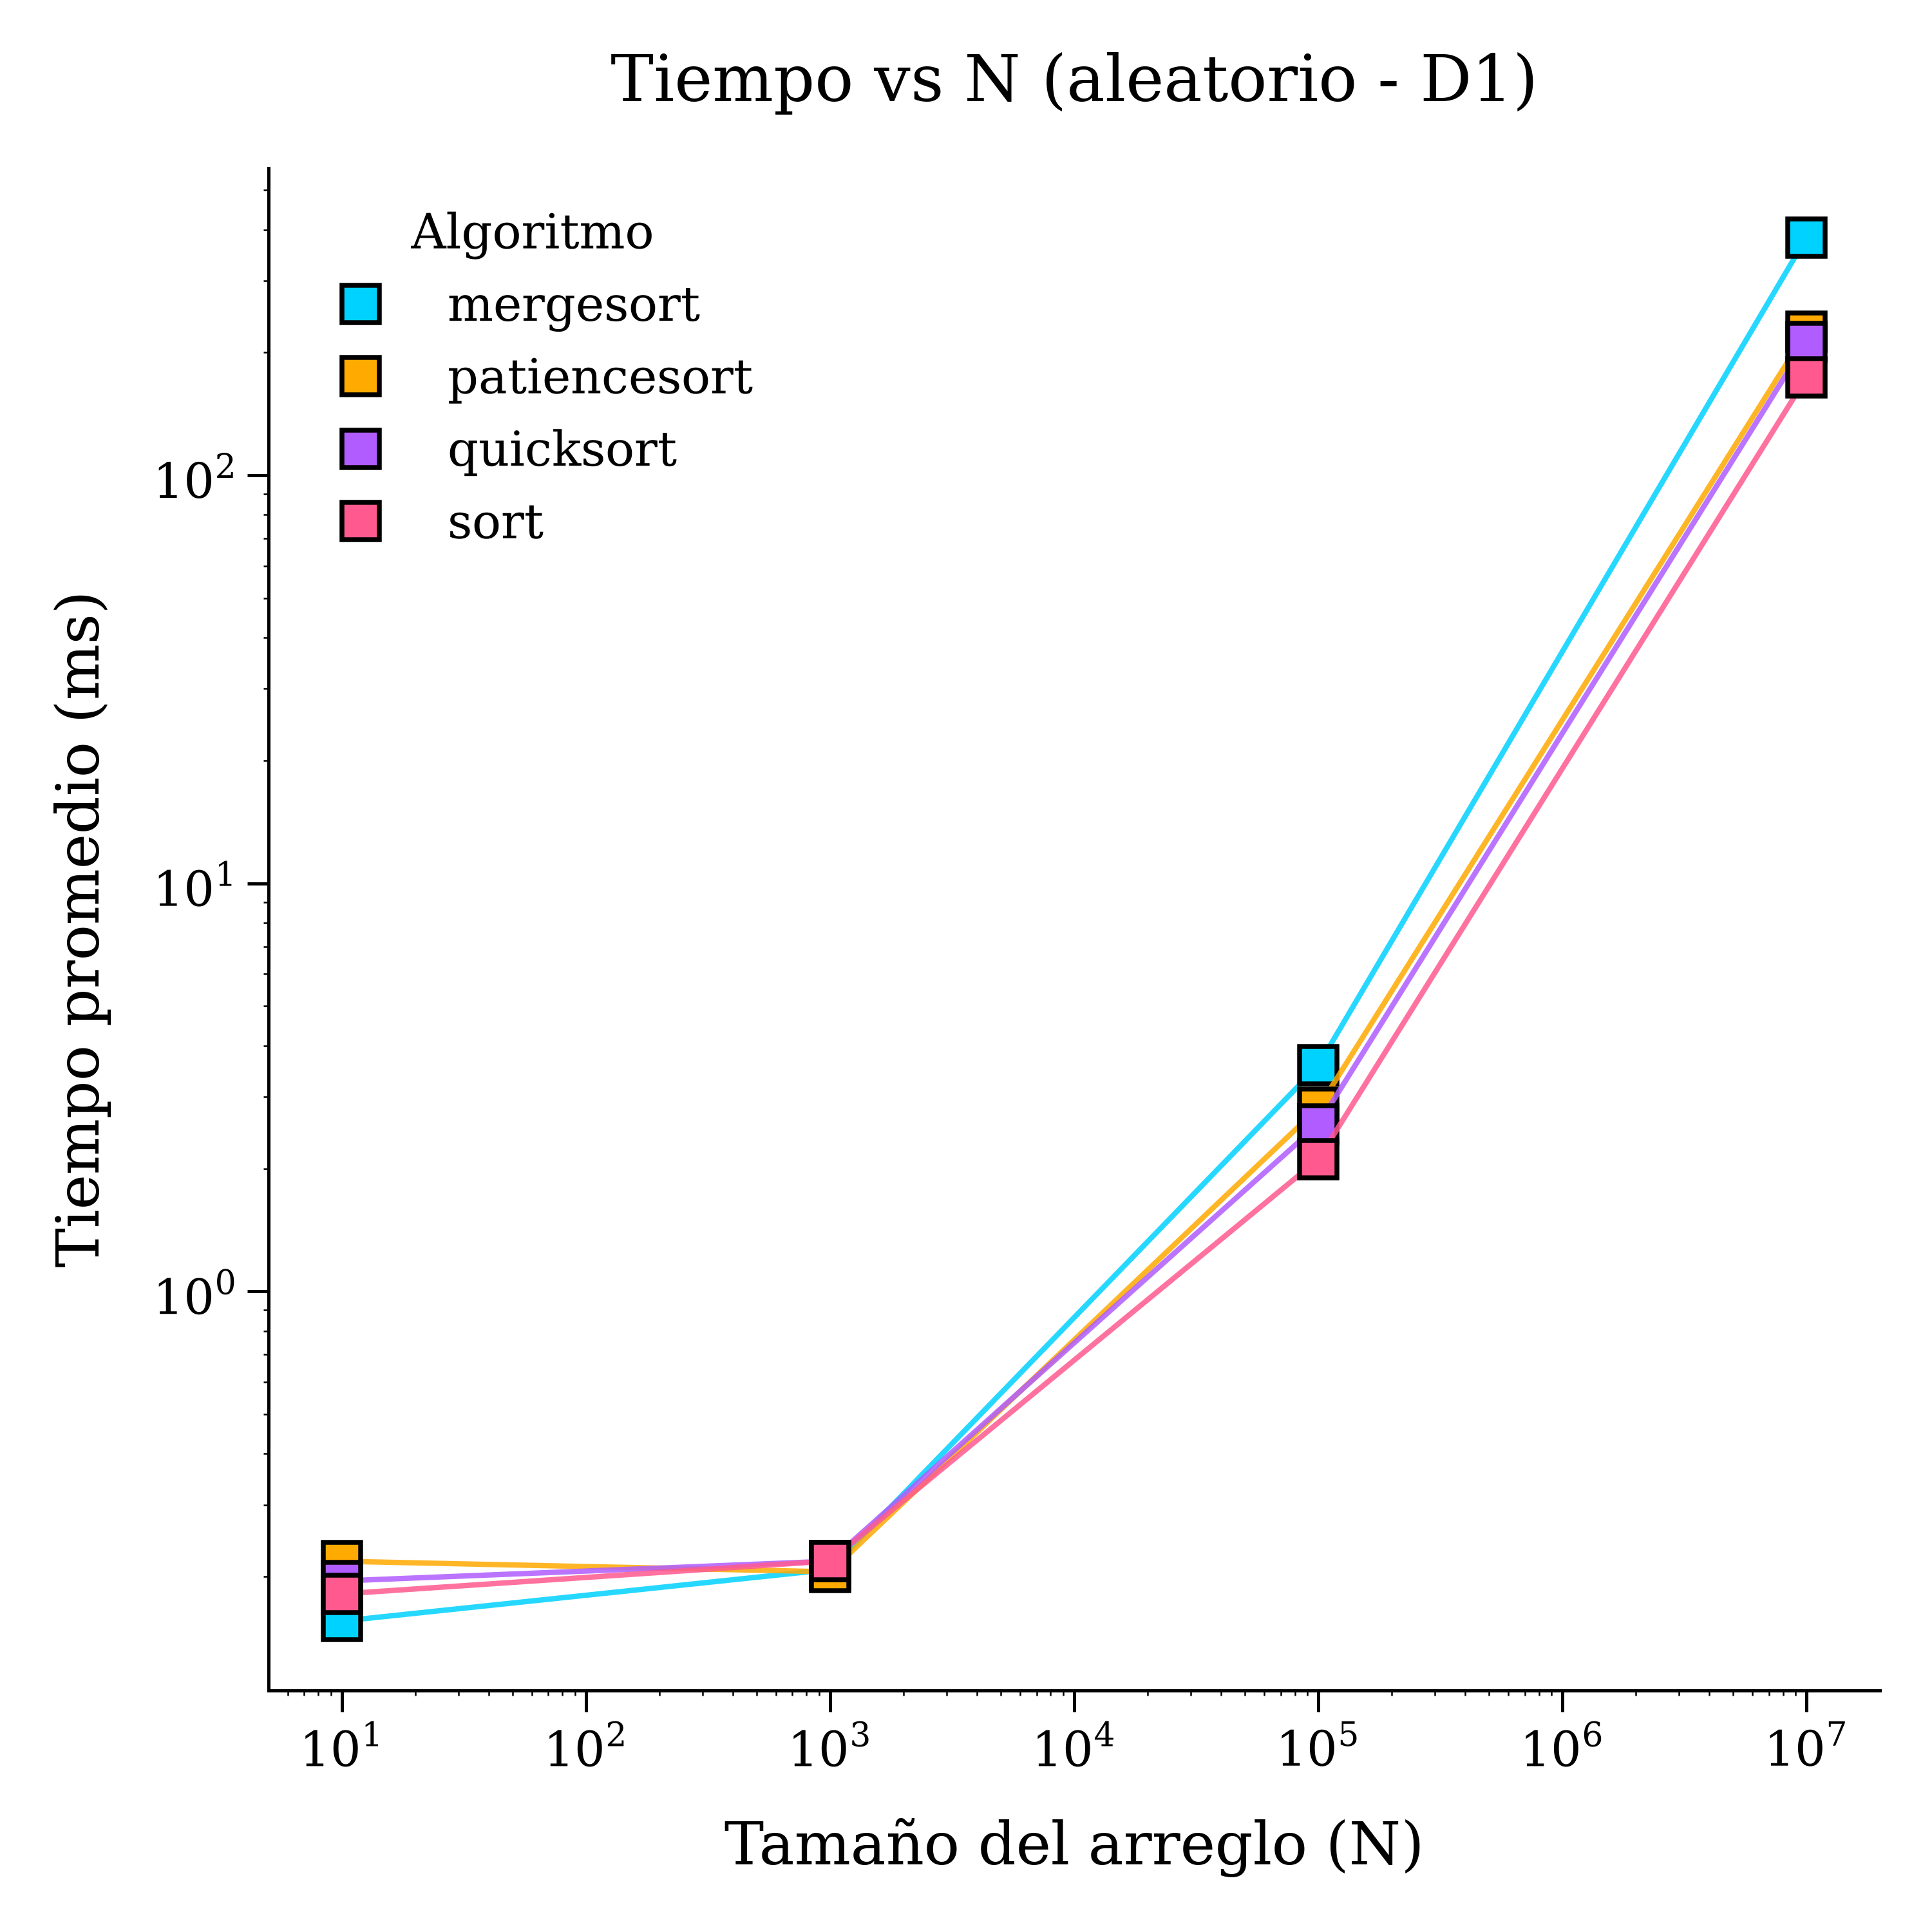
\includegraphics[width=0.48\textwidth]{../code/sorting/data/plots/sorting_aleatorio_D1.png}%
    }
    \hfill
    \subfloat[Aleatorio - Dominio $D_7$]{%
        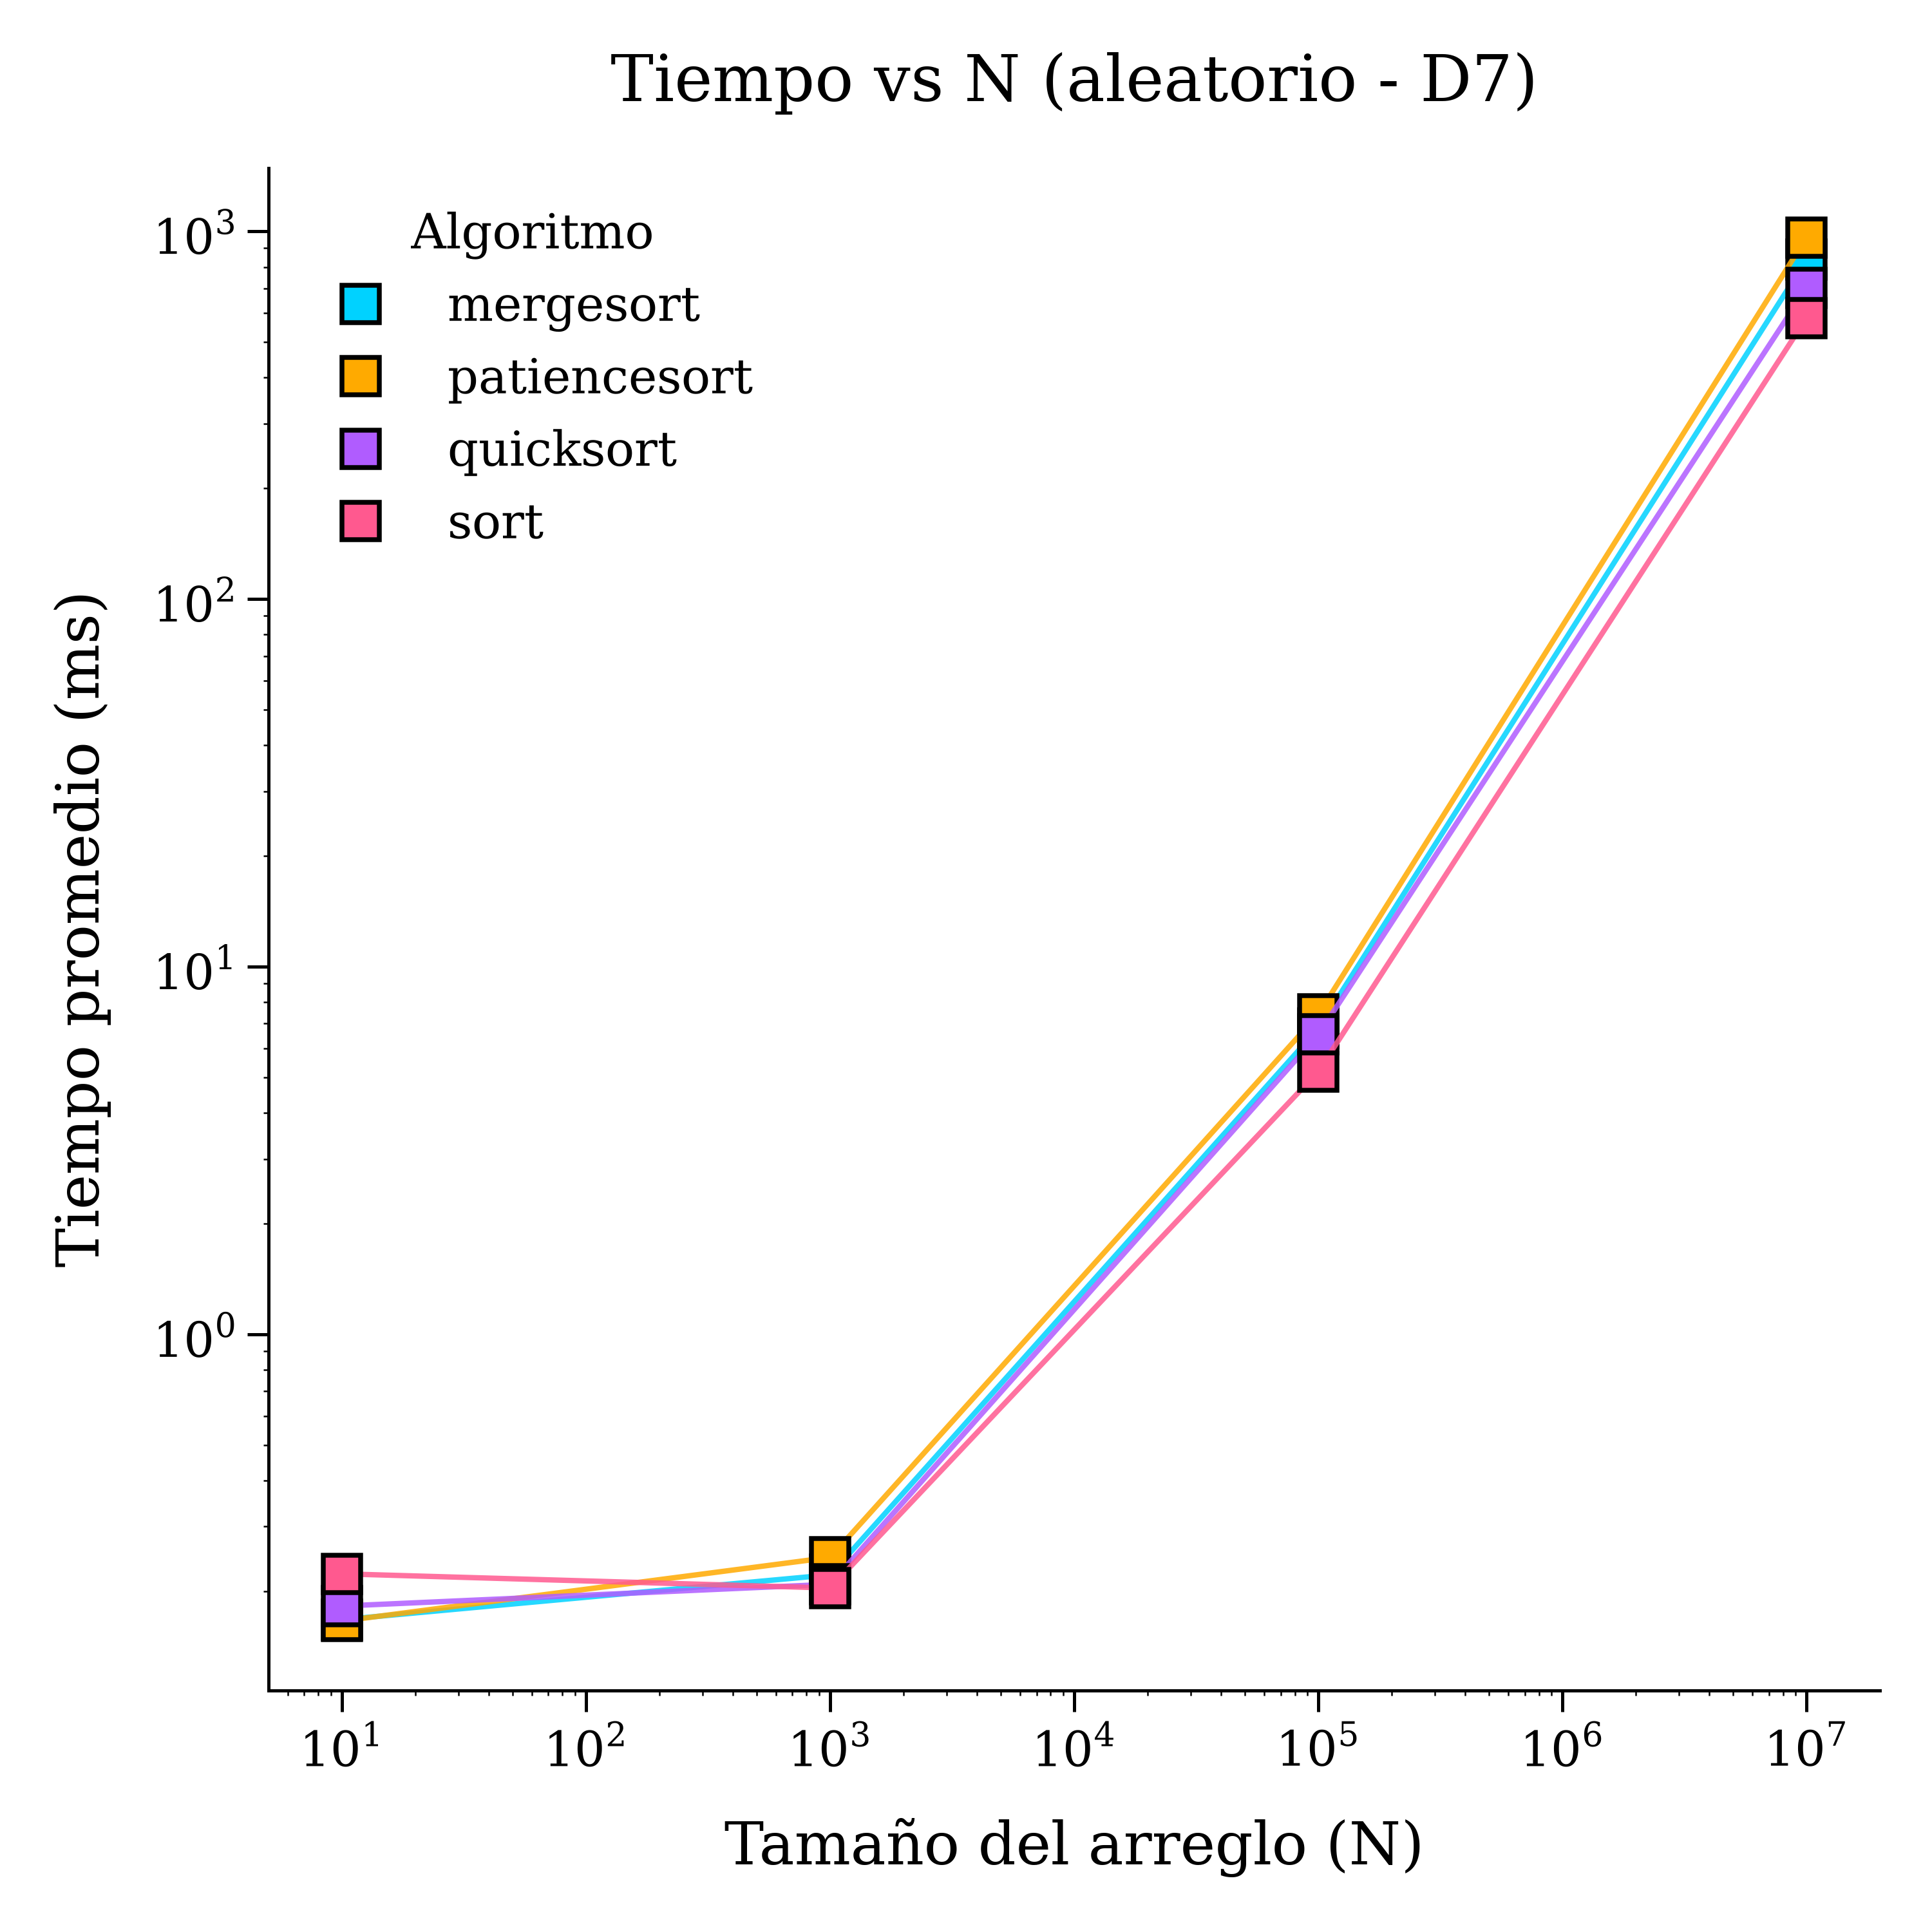
\includegraphics[width=0.48\textwidth]{../code/sorting/data/plots/sorting_aleatorio_D7.png}%
    }
    \caption{Tiempos de ejecución en ordenamiento para datos aleatorios en dominios $D_1$ y $D_7$.}
    \label{fig:sorting_plots}
\end{figure}

Como se aprecia empíricamente, \texttt{std::sort} (implementación introspectiva híbrida) lidera consistentemente en tiempo de CPU. En el dominio $D_1$, donde el rango de valores posibles es diminuto ($[0,9]$) y abundan las colisiones, todos los algoritmos experimentan una notable reducción de tiempo respecto a $D_7$. QuickSort mantiene un desempeño sumamente competitivo gracias a su excelente localidad espacial de caché. Por su parte, PatienceSort exhibe un comportamiento particular: ante entradas ordenadas o con claves altamente concentradas ($D_1$), el número de pilas que mantiene es bajo, minimizando las comparaciones en la búsqueda binaria; sin embargo, en $D_7$ con valores crecientes o aleatorios, la cantidad de pilas se aproxima a $N$, encareciendo la fase de reconstrucción por montículo.

\subsection{Multiplicación de Matrices Cuadradas}

La \Cref{tab:matrix_summary} resume los tiempos promedio de ejecución para matrices densas en dominio $D_{10}$, mientras que la \Cref{fig:matrix_plots} presenta las curvas comparativas entre ambos algoritmos en escala logarítmica.

\begin{table}[H]
\centering
\caption{Tiempo de ejecución promedio (ms) para multiplicación de matrices densas ($D_{10}$).}
\label{tab:matrix_summary}
\small
\begin{tabular}{rrrr}
\hline
\textbf{Dimensión ($N$)} & \textbf{Naive (ms)} & \textbf{Strassen (ms)} & \textbf{Ratio (Strassen / Naive)} \\ \hline
16   & 0.0035 ms & 1.3288 ms   & $\approx 379\times$ \\
64   & 0.0570 ms & 62.3046 ms  & $\approx 1093\times$ \\
256  & 3.5297 ms & 3838.94 ms  & $\approx 1087\times$ \\
1024 & 155.53 ms & 152541.3 ms & $\approx 980\times$ \\ \hline
\end{tabular}
\end{table}

\begin{figure}[H]
    \centering
    \subfloat[Matrices Densas - Dominio $D_{10}$]{%
        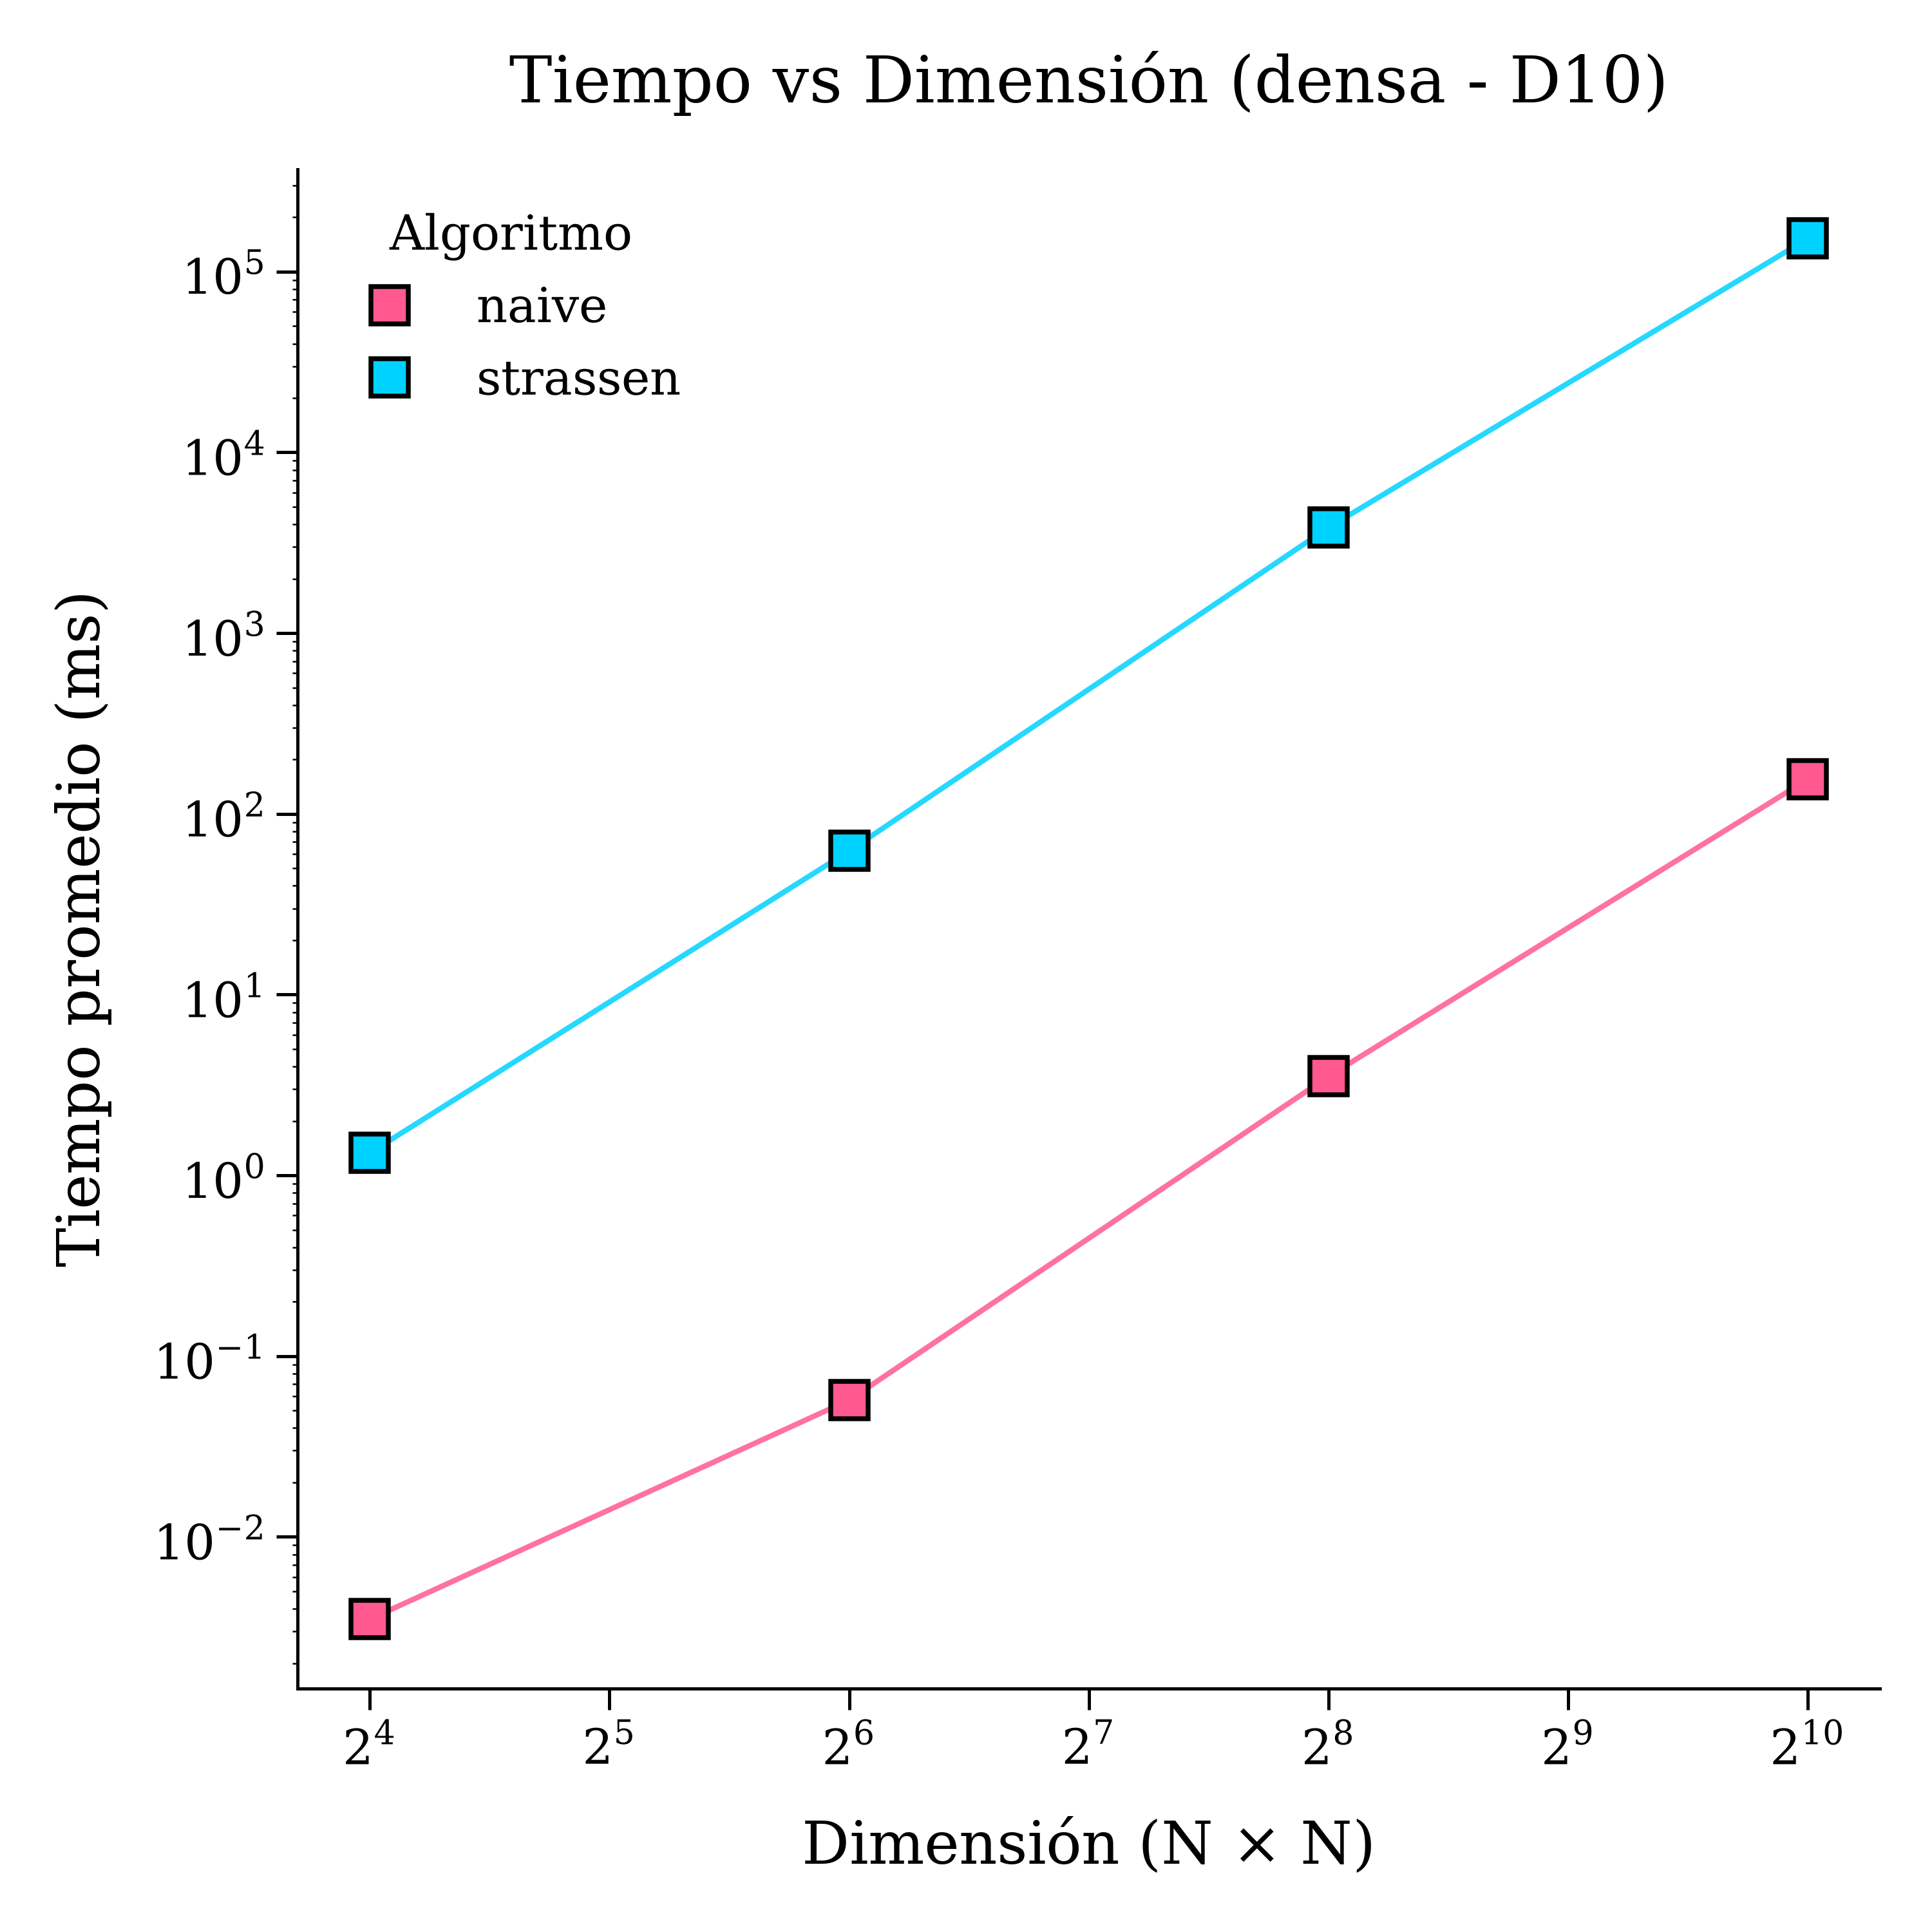
\includegraphics[width=0.48\textwidth]{../code/matrix_multiplication/data/plots/matrix_densa_D10.png}%
    }
    \hfill
    \subfloat[Matrices Dispersas - Dominio $D_0$]{%
        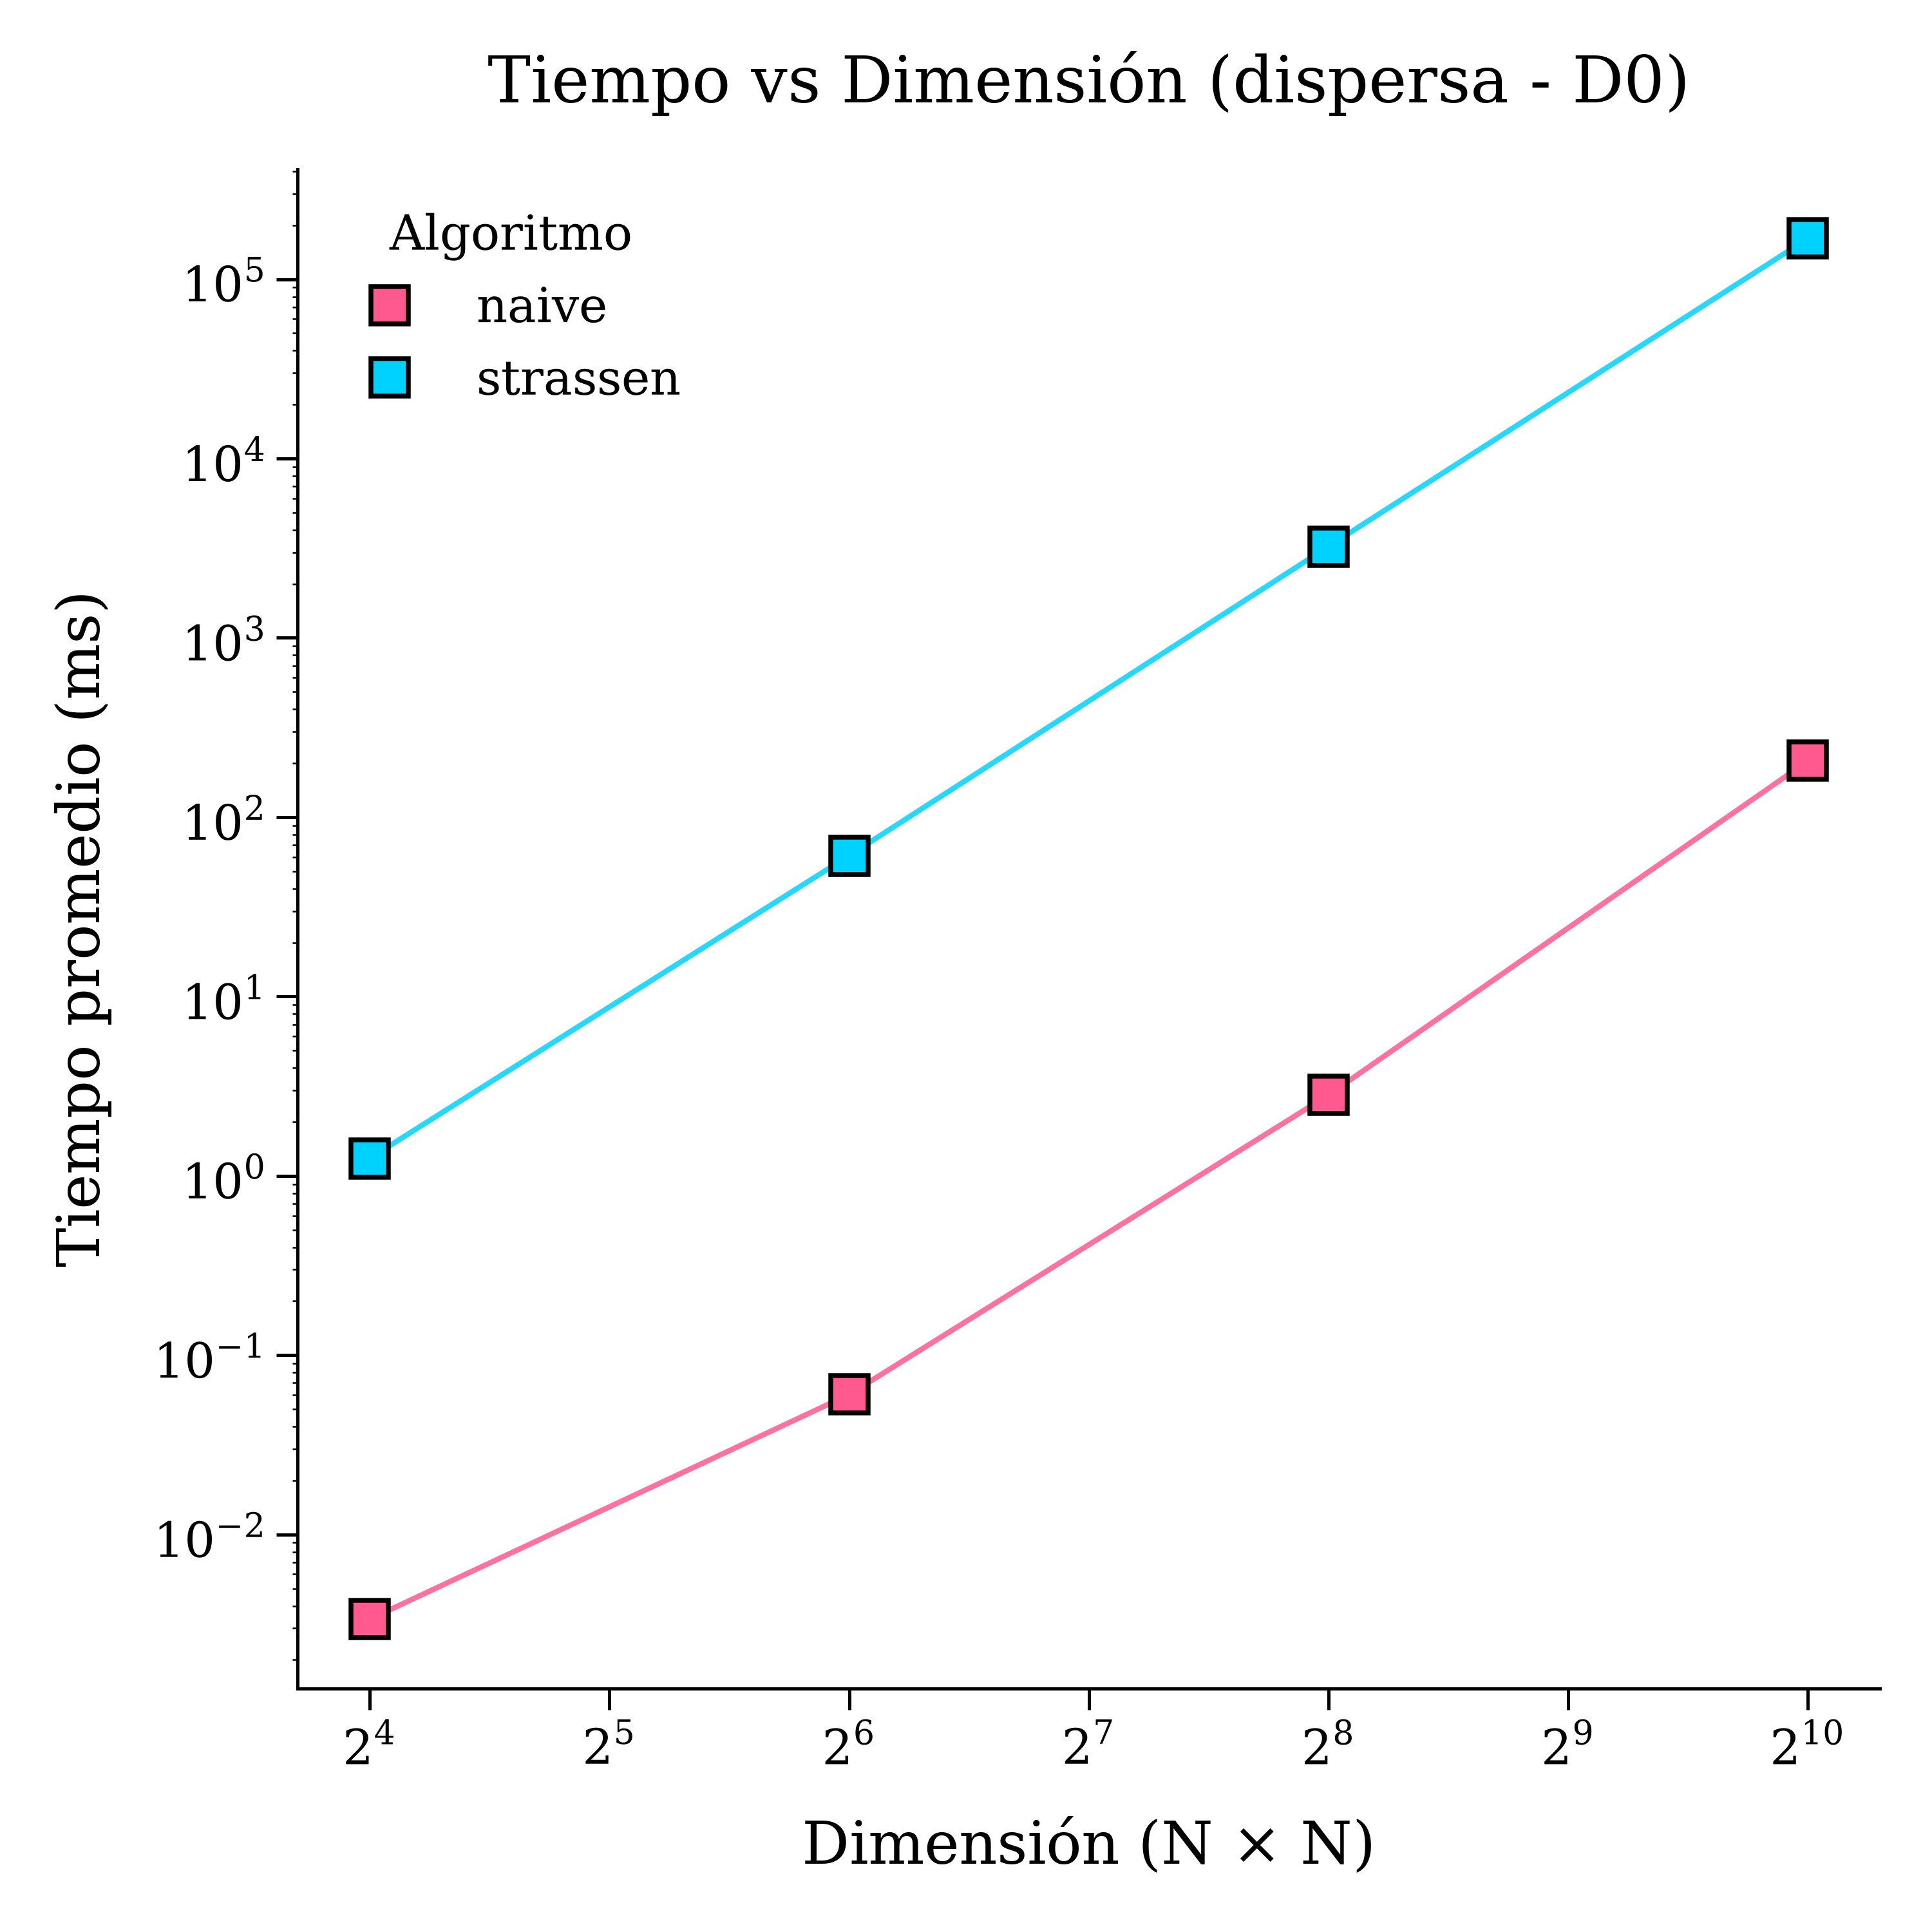
\includegraphics[width=0.48\textwidth]{../code/matrix_multiplication/data/plots/matrix_dispersa_D0.png}%
    }
    \caption{Desempeño empírico en multiplicación matricial (Naive vs. Strassen).}
    \label{fig:matrix_plots}
\end{figure}

Aunque en la teoría matemática Strassen promete ser más rápido que Naive porque realiza menos multiplicaciones ($\mathcal{O}(N^{2.81})$ contra $\mathcal{O}(N^3)$), en las pruebas prácticas ocurrió lo contrario: Naive fue drásticamente más veloz, llegando a ser casi 1000 veces más rápido en matrices de $1024 \times 1024$ (0.15 segundos frente a más de 2.5 minutos de Strassen). 

Esta gran diferencia se debe principalmente a cómo trabaja la computadora en la realidad:
\begin{enumerate}[leftmargin=1.5em, itemsep=1pt]
    \item \textbf{Naive es simple y ordenado para el procesador:} Utiliza bucles directos sobre memoria continua. Al compilar con la bandera \texttt{-O3}, la computadora puede leer y multiplicar varios números al mismo tiempo aprovechando la memoria rápida (caché) sin interrupciones.
    \item \textbf{Strassen tiene demasiado trabajo extra (sobrecarga):} Al ser recursivo, parte las matrices en pedazos pequeños una y otra vez. En cada división debe crear y borrar decenas de matrices temporales en la memoria RAM. Ese constante proceso de pedir y liberar memoria hace que el procesador gaste la mayor parte del tiempo organizando datos en vez de multiplicarlos.
\end{enumerate}